\documentclass[11pt, a4paper]{report}
\usepackage[T2A]{fontenc}
\usepackage{graphicx}
\usepackage{multirow}
\usepackage[left=2.5cm, right=2cm, top=2cm, bottom=2cm]{geometry}
\usepackage{fontspec}
\usepackage{titlesec}
\usepackage{setspace}
\usepackage{lipsum}
\usepackage{indentfirst}
\usepackage{tabularx}
\usepackage{array}
\usepackage{multirow}

\setmainfont{Times New Roman}

\graphicspath{{images}}

\newcommand{\Nmct}{{Шинэ Монгол Технологийн Коллеж}}
\newcommand{\Major}{{Конпьютерийн Ухааны Тенхим}}
\newcommand{\Robocon}{{ABU Робокон 2026}}
\newcommand{\Title}{{ABU Робокон 2026 тэмцээний бүрэн автомат роботын программчлал}}
\newcommand{\rownum}{\stepcounter{rownum}\arabic{rownum}}
\newcommand{\rownumreset}{\setcounter{rownum}{0}}

\renewcommand{\contentsname}{Агуулга}
\renewcommand{\figurename}{Зураг}
\renewcommand{\tablename}{Хүснэгт}
\renewcommand{\listtablename}{Хүснэгтийн жагсаалт}
\renewcommand{\listfigurename}{Зургийн жагсаалт}
\renewcommand{\bibname}{Ном зүй}

\titleformat{\chapter}[hang]
	{\bfseries\huge}
	{\thechapter.}
	{1em}
	{}
	
\begin{document}
	\newcounter{rownum}

	\singlespacing{}
	\pagestyle{empty}
	
	% Title page
	\begin{minipage}[h]{0.2\textwidth}
		
\includegraphics[width=\textwidth]{nmct_logo.png}
	\end{minipage}
	\hfill
	\begin{minipage}[h]{0.7\textwidth}
		\centering
		\large
		\MakeUppercase{\textbf{
			\Nmct{} \\[3mm]
			\Major{}
		}}
	\end{minipage}

	\vspace{4cm}
	\begin{flushright}
		\large
		\begin{tabular}{r l}
			Оюутны код: & s21c019b \\[5mm]
			Оюутны нэр: & М. Молор
		\end{tabular}
	\end{flushright}

	\vspace{4cm}
	\begin{center}
		{\MakeUppercase{
			\textbf{\Large \Title{}} \\[5mm]
			 /Дэд бакалаврын төгсөлтийн судалгааны ажил/
		}}
		
		\vspace{5mm}
		\large
		\begin{tabular}{l r}
			Удирдсан багш: & У. Анужин /Магистрат/ \\[5mm]
			Гүйцэтгэсэн оюутан: & М. Молор
		\end{tabular}
	\end{center}

	\vspace{\fill}
	\begin{center}
		Улаанбаатар хот \\
		2025 он
	\end{center}
	
	% Title 2

	\newpage
	\begin{center}
		\Large
		\Nmct{} \\[5mm]
		\Major{}
		
		\vspace{6cm}
		Төгсөлтийн судалгааны ажил (Мэргэжлийн индекс) \\[5mm]
		\textbf{\Title{}}
		
		\large
		\vspace{3cm}
		\begin{tabular}[h]{r l}
			Гүйцэтгэгч: & М. Молор \\[5mm]
			Удирдагч: & У. Анужин
		\end{tabular}
		
		\vspace{\fill}
		Улаанбаатар хот \\
		2025 он
	\end{center}

	% Roman numbering
	\newpage
	\pagestyle{plain}
	\pagenumbering{roman}
	\setcounter{page}{1}
	
	% Huraangui
	\addcontentsline{toc}{chapter}{Хураангуй}

	\begin{center}
		\MakeUppercase{\textbf{\Large \Title{}}}

		\vspace{5mm}
		М. Молор \\
		\Nmct{}, \Major{} \\
		\textit{s21c019b@nmct.edu.mn}
	\end{center}

	\vspace{5mm}
	\noindent
	\textbf{Хураангуй:}
	ABU Робокон тэмцээн нь жил бүр их сургуулиудад зохион байгуулагддаг тэмцээн бөгөөд, энэхүү тэмцээнээр багууд дүрмийн дагуу даалгавар биелүүлэх чадвартай робот угсарч, өрсөлдөгч багтай уралдаж тоглодог тэмцээн юм.

	Энэ жилийн тэмцээн нь R1 болон R2 гэсэн 2 робот угсарч, өрсөлдөх бөгөөд, R1 робот нь удирдлагатай байж болох ч, R2 нь бүрэн автомат байх ёстой юм. Энэ нь дүрс таних, шийдвэр гаргах, саад бартаа туулах зэрэг компьютерын ухааны салбартай холбоотой олон төрлийн алгоритмын программчлал шаардагдах тул энэхүү судалгааны ажилын хүрээнд дүрс таних болон шийдвэр гаргах шийдлүүдийг судалсан болно.

	\vspace{10mm}
	\noindent
	\textbf{Түлхүүр үг:} \textit{Робокон, Дүрс таних, Шийдвэр гаргах, Робот}

	% LOF/LOT
	\listoffigures
	\addcontentsline{toc}{chapter}{Зургийн жагсаалт}
	\listoftables
	\addcontentsline{toc}{chapter}{Хүснэгтийн жагсаалт}
	
	% TOC
	\tableofcontents
	\thispagestyle{empty}
	
	\newpage
	\chapter{Удиртгал}

\pagestyle{plain}
\pagenumbering{arabic}
\setcounter{page}{1}

\section{Ажлын Төлөвлөгөө}

\begin{table}[h]
    \centering
    \begin{tabular}{|c|c|l|}
        \hline
        Сар & Долоо хоног & Төлөвлөгөө \\ \hline
        \multirow{4}{*}{10 сар} & 1 & Робоконы дүрэмтэй танилцах \\ \cline{2-3}
        & 2 & Тоглолтын стратеги боловсруулах \\ \cline{2-3}
        & 3 & Онолын судалгаа хийх \\ \cline{2-3}
        & 4 & Симуляцийн модель үүсгэх \\ \hline
        \multirow{4}{*}{11 сар} & 1 & Датасет боловсруулах \\ \cline{2-3}
        & 2 & Дүрс таних алгоритмын судалгаа \\ \cline{2-3}
        & 3 & Судар таних алгоритмын хөгжүүлэлт, сургалт \\ \cline{2-3}
        & 4 & Туршилт, үр дүн \\ \hline
        \multirow{4}{*}{12 сар} & 1 & \textbf{ТСА Үзлэг 1} \\ \cline{2-3}
        & 2 & Шийдвэр гаргах алгоритмын судалгаа \\ \cline {2-3}
        & 3 & Шийдвэр гаргах алгоритм хөгжүүлэлт \\ \cline {2-3}
        & 4 & Туршилт, үр дүн \\ \hline
        \multirow{4}{*}{1 сар} & 1 & Икс Окс таамаглах алгоритмын судалгаа \\ \cline{2-3}
        & 2 & Алгоритмын хөгжүүлэлт \\ \cline{2-3}
        & 3 & Икс окс тоглоомын дүрс таних алгоритмын судалгаа \\ \cline{2-3}
        & 4 & Алгоритмын хөгжүүлэлт, сургалт \\ \hline
        \multirow{4}{*}{2 сар} & 1 & Систем нэгтгэх \\ \cline{2-3}
        & 2 & Роботын программчлал \\ \cline{2-3}
        & 3 & Системийн суурилуулалт \\ \cline{2-3}
        & 4 & Роботын туршилт \\ \hline
        \multirow{4}{*}{3 сар} & 1 & \textbf{ТСА Үзлэг 2} \\ \cline{2-3}
        & 2 & Сайжруулсан алгоритм сургах \\ \cline{2-3}
        & 3 & Бодит амьдрал дээр турших \\ \cline{2-3}
        & 4 & Роботын программчлал \\ \hline
        \multirow{4}{*}{4 сар} & 1 & Тэмцээнд оролцох \\ \cline{2-3}
        & 2 & Хураангуй бичих \\ \cline{2-3}
        & 3 & Бичвэрийн эцсийн хувилбар \\ \cline{2-3}
        & 4 & \multirow{3}{*}{\textbf{ТСА урьдчилсан хамгаалалт}} \\ \cline{1-2}
        \multirow{4}{*}{5 сар} & 1 & \\ \cline{2-2}
        & 2 & \\ \cline{2-3}
        & 3 & \multirow{2}{*}{\textbf{ТСА үндсэн хамгаалалт}} \\ \cline{2-2}
        & 4 & \\ \hline
    \end{tabular}
    \caption{Ажлын төлөвлөгөө}
    \label{table:plan}
\end{table}

\newpage

\section{Үндэслэл, ач холбогдол}
ABU Робокон 2026 тэмцээн нь багаараа робот угсарч, өрсөлдөгч багийн роботтой уралддаг тэмцээн юм. Энэ тэмцээнээр R1 болон R2 гэх роботууд угсрах шаардлагатай бөгөөд, R1 робот нь хүний удирдлагаар ажиллах робот бол R2 робот нь бүрэн автомат робот байх ёстой.

Иймд энэхүү судалгааны ажил нь тэмцээнд ашиглагдах R2 бүрэн автомат роботын программчлалын аргачлал, шийдэл болон түүнийг хэрэгжүүлэхэд шаардлагатай онолын болон практик талаас нь судлахад чиглэнэ.

\section{Зорилго, зорилт}

\subsection{Зорилго}
Энэхүү судалгааны ажил нь Робокон 2026 тэмцээнд дүрмийн дагуу даалгавраа гүйцэтгэх чадвартай R2 бүрэн автомат роботын удирдлагын системийг программчлах зорилготой юм.

\subsection{Зорилт}
\begin{enumerate}
    \item Робокон тэмцээний дүрэмтэй танилцах
    \item Симуляцийн орчин үүсгэх
    \item Сургалтын датасет үүсгэх
    \item Судар таних систем сургалт
    \item Икс окс тоглох систем сургалт
    \item Байршил тогтоох систем хөгжүүлэлт
    \item Шийдвэр гаргах систем хөгжүүлэлт
    \item Сайжруулалт
\end{enumerate}

	
	% Onol
	\chapter{Онолын судалгаа}
\section{Робоконий дүрэм}
Робоконий тоглох зааланд 2 баг өрсөлдөх бөгөөд, баг тус бүрд заалын тэн хагас нь оноогдоно. Мөн оноогдсон хэсэг тус бүр нь дотроо 3 zone-д хуваагдах бөгөөд, тэдгээр нь:
\begin{itemize}
    \item Martial club --- Тулааны клуб
    \item Meihua forest --- Мэйхуа ой
    \item Arena --- Тулааны талбар
\end{itemize}
нэртэй байна.

\begin{figure}[h]
    
\includegraphics[width=1\textwidth]{robocon_field.png}
    \caption{\Robocon{} тэмцээний тоглох талбай}
    \label{fig:robocon_field}
\end{figure}

\newpage

Нэг багаас 2 робот өрсөлдөх бөгөөд, үүнд:
\begin{itemize}
    \item R1 робот --- Удирдлагатай эсвэл автомат байж болно.
    \item R2 робот --- Бүрэн автомат байх бөгөөд ямар ч комманд болон удирдлага авахгүй байна.
\end{itemize}

Мөн Мэйхуа ой дээр 8 ширхэг Күнгфү судар (Kung fu scroll) байрлуулна. Үүнд:
\begin{itemize}
    \item 3 ширхэг R1-ийн судар нь R1 робот авахад зориулсан байх бөгөөд, бүх талдаа тэнцээний логотой байна.
    \item 4 ширхэг R2-ийн судар нь R2 робот авахад зориулсан байх бөгөөд, бүх талдаа жинхэнэ мэргэний ясан бичиг агуулсан байна.
    \item Үлдсэн нэг нь хуурамч судар байх ба, аль ч робот авах ёсгүй байхаар, бүх талдаа хуурамч мэргэний ясан бичигтэй байна.
\end{itemize}
Дүрэм дээр жинхэнэ болон хуурамч мэргэний ясан бичиг тус бүр 15 ширхэг байх ба тэмцээний үеэд эдгээрээс 7 ширхэг жинхэнэ, 1 ширхэг хуурмаг бичиг дурын сонгогдож, Күнгфү сударт бичигдэнэ.

\begin{figure}[h]
    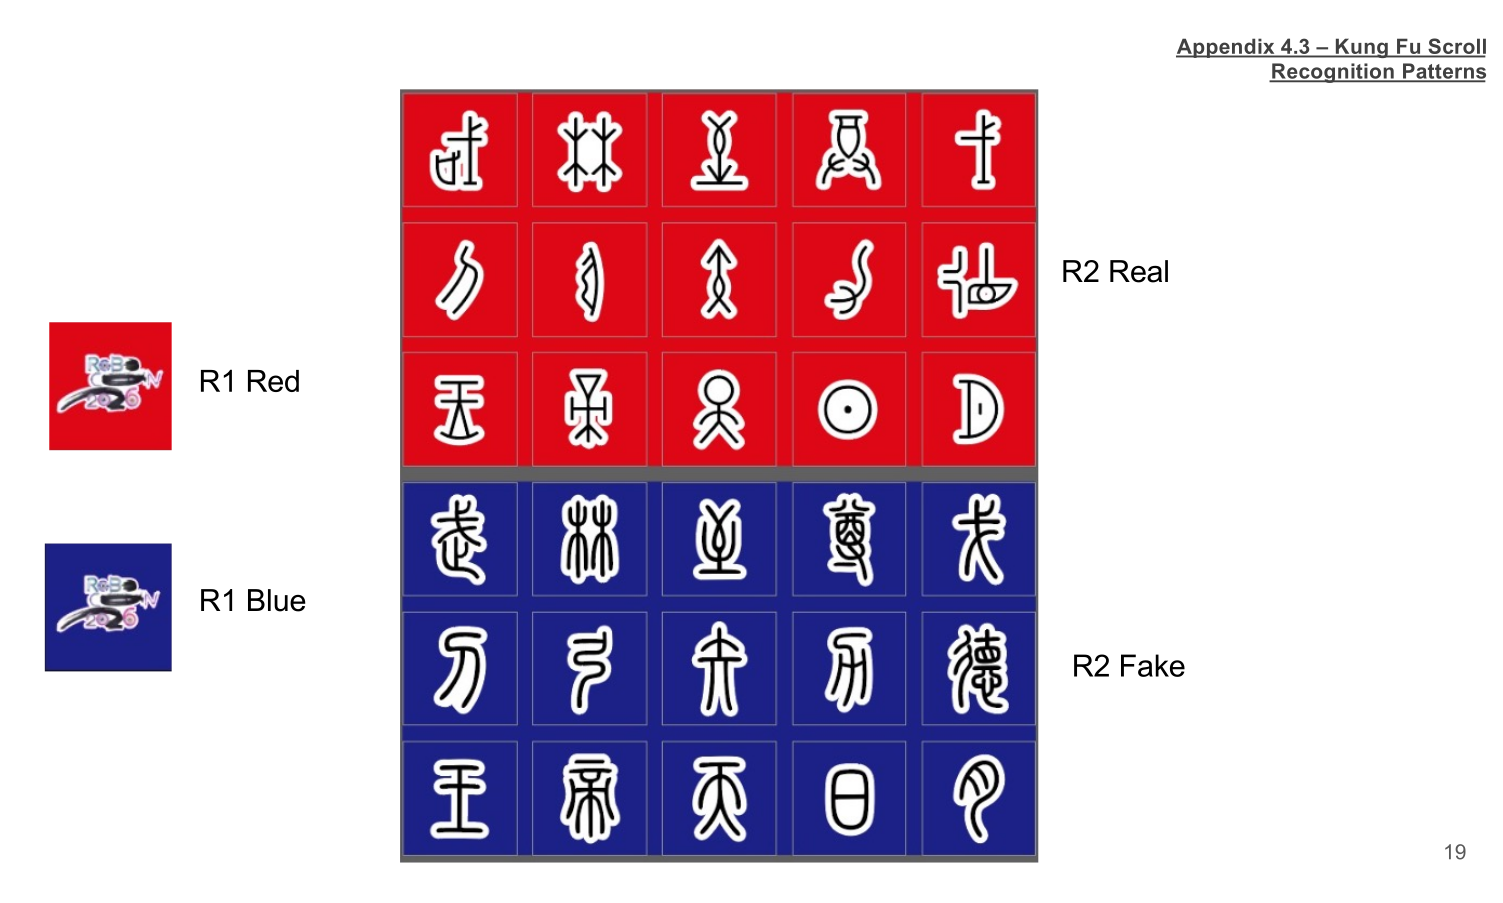
\includegraphics[width=\textwidth]{robocon_kfs.png}
    \caption{\Robocon{} тэмцээний Күнгфү сударт тавигдах дүрсүүд.}
    \label{fig:robocon_kfs}
\end{figure}

\subsection{Тулааны клуб zone}
Тулааны клуб zone-оос роботууд хөдөлж эхлэх бөгөөд, роботоо бэлдэх 1 минут өгнө.

\newpage
\section{Күнгфү судар таних}

Күнгфү судар танихад зураг таних машин сургалт хэрэгтэй болно. Сургахад бодит дата одоогоор байхгүй байгаа тул симуляцийн орчинд күнгфү сударуудыг үүсгэж, датасэт үүсгэх хэрэгтэй болж байна.

Мөн күнгфү судар нь 15 үнэн болон 15 хуурмаг бичиг байгаа бөгөөд, \Robocon{} тэмцээний логотой судар гэх 3 төрлийн датасет сургах хэрэгтэй болно. Учир нь R2 робот буруу судараа ерөнхийд нь ойролцоо гэж таних магадлалтай тул буруу сударуудыг нь заавал таниулж, авахгүй байх зориулалттай байна.

\subsection{Датасет боловсруулах}

Датасет боловсруулахад Unity гэх видео тоглоом хийхэд зориулсан систем ашиглаж, симуляцийн орчин үүсгэж, датасетээ боловсруулна.

Unity нь 2 хэмжээст болон 3 хэмжээст видео тоглоом хийхэд зориулагдсан game engine юм. Unity нь өндөр чанартай бодит амьдралтай ойролцоо гэрэлтүүлэг, сүүдэр, камерийн эффект тохируулснаар, янз бүрийн гэрэлтүүлэг, сүүдэр, бүрэлзэх, г.м. тохиолдлуудыг симуляц хийж, өндөр чанартай сургалтын датасет боловсруулах чадвартай байна.

\begin{figure}[h]
    \centering
    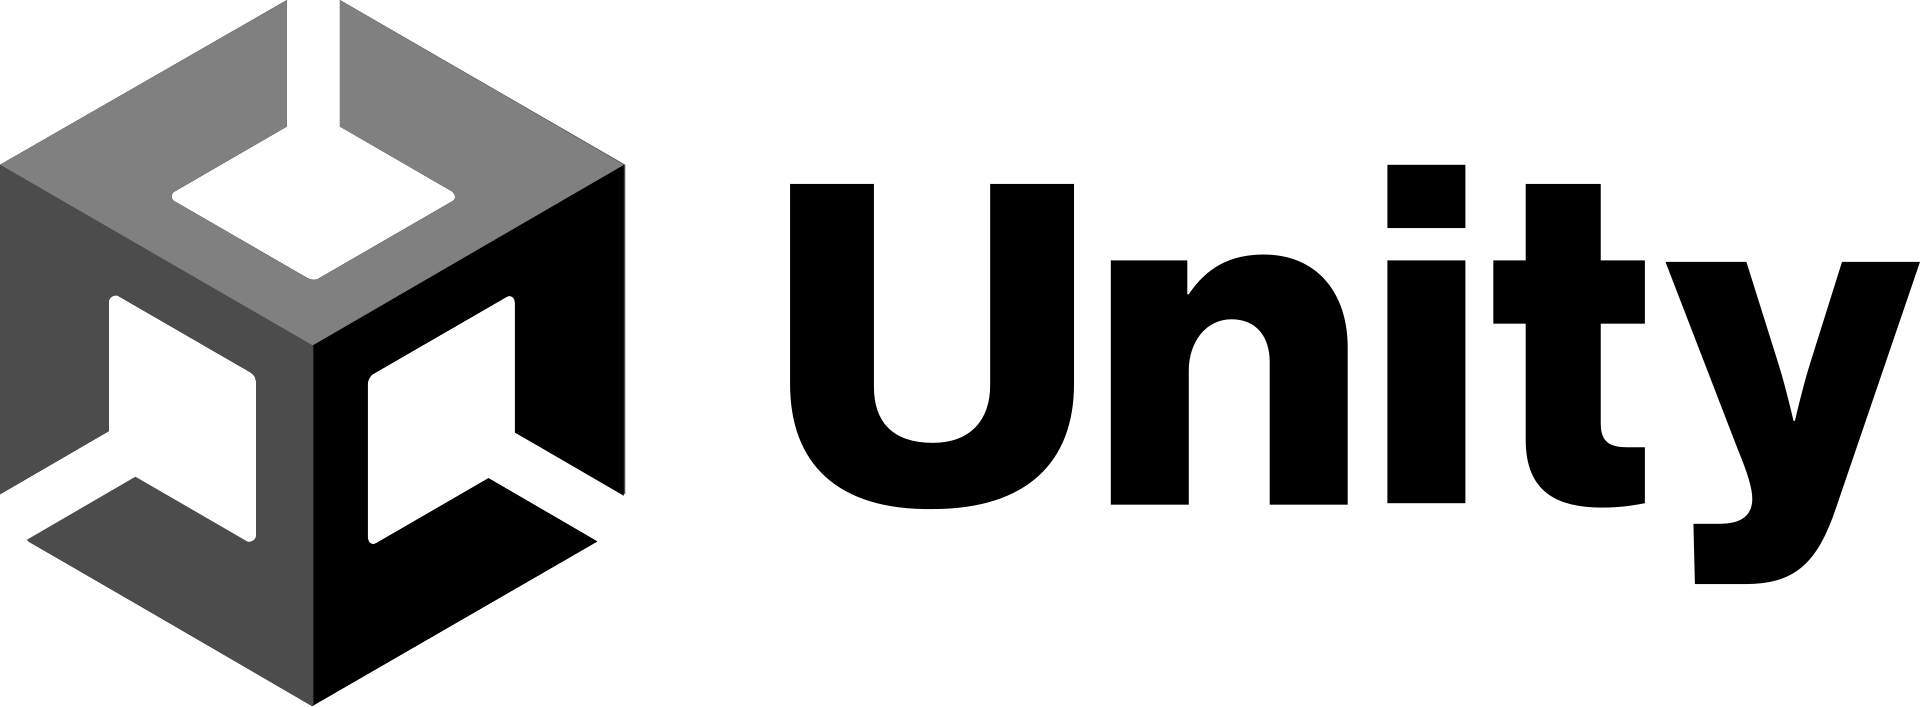
\includegraphics[width=0.5\textwidth]{unity.png}
    \caption{Unity Game Engine лого}
    \label{fig:unity}
\end{figure}

\subsection{Модель үүсгэх}

Симуляцийн орчин бүрдүүлэхэд тоглох талбай болон судруудын модель үүсгэх хэрэгтэй.

Тоглох талбайн хэмжээ нь дүрэм дээр өгөгдсөн байгаа бөгөөд, талбайг загварчлахдаа FreeCAD ашиглсан загварчилсан болно.

\begin{figure}[h]
    \centering
    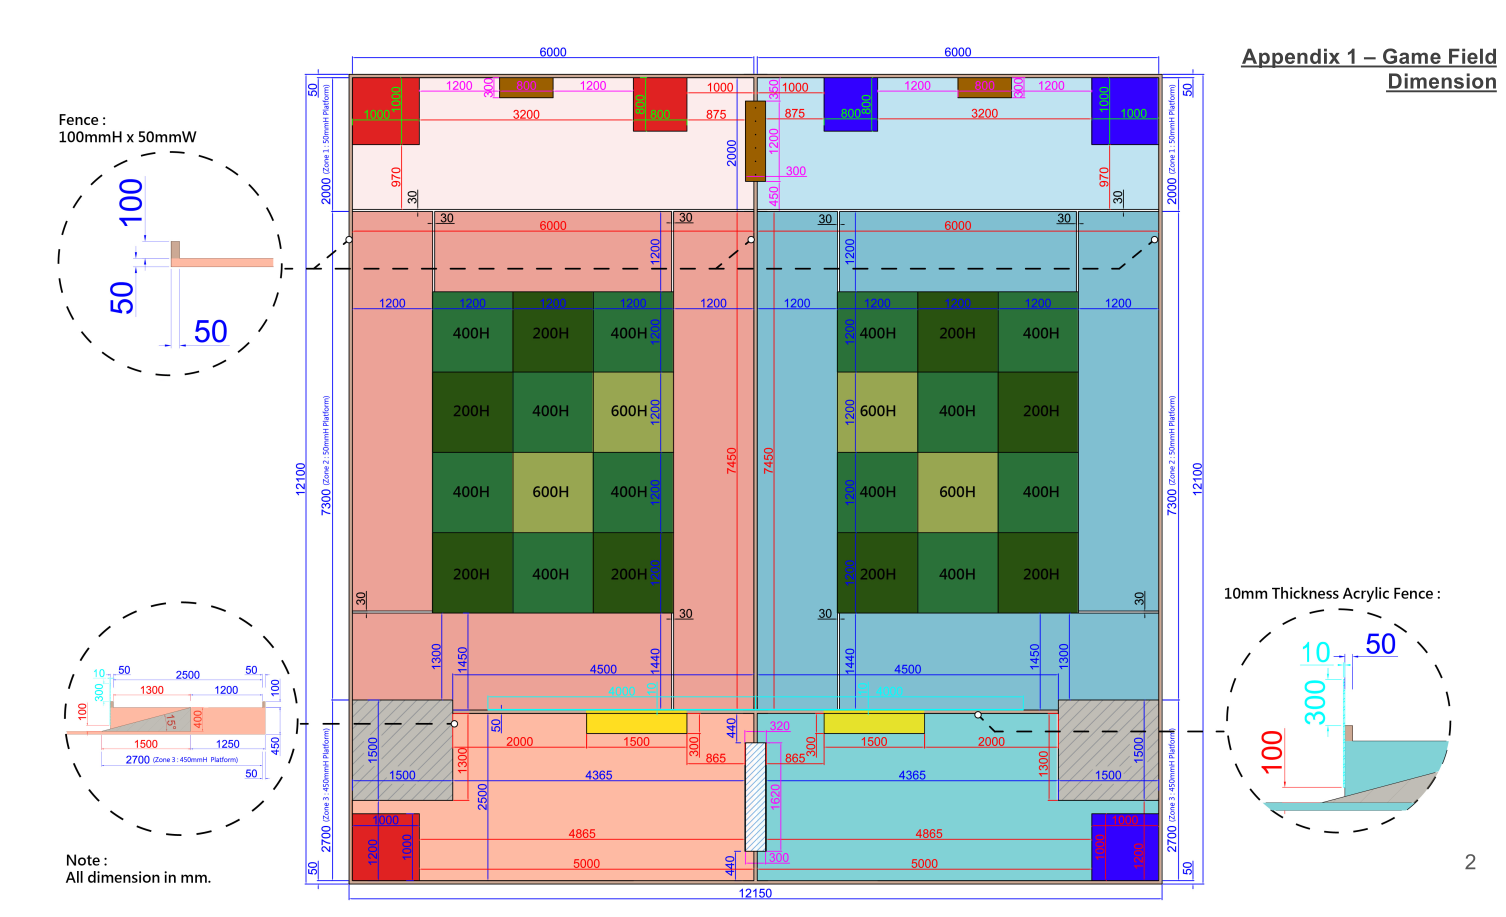
\includegraphics[width=\textwidth]{robocon-field-blueprint.png}
    \caption{Робокон тэмцээний дүрэм дээр заасан тоглох талбайн хэмжээ}
    \label{fig:field-blueprint}
\end{figure}
\begin{figure}[h]
    \centering
    
\includegraphics[width=0.7\textwidth]{logo-freecad.png}
    \caption{FreeCAD лого}
    \label{fig:freecad}
\end{figure}

FreeCAD нь математик тооцооллоор геометр дүрсүүд ашиглан биет бүтээдэг билээ. Гэвч Unity нь зөвхөн гурвалжин дүрсээр бүрдэх торон бүтэцтэй биетийг зурах чадвартай байдаг байна. Үүнд зориулсан гурвалжин торлог бүтэц агуулах файлын формат төрөл бүр байдаг бөгөөд, өргөн хэрэглэгддэг .stl болон .fbx форматуудыг ашигласан болно.

.stl формат нь FreeCAD программын үүсгэж чадах формат бөгөөд, торон биетийн гурвалжин бүрийн өнцгүүдийн координатыг хадгалдаг формат юм.

.fbx формат нь .stl форматтай адил торон биетийн бүтцийг хадгалахаас гадна тухайн биет ямар өнгөтэй, гэрлэнд ойх чанар, барзгар болон тэгш гадаргуу г.м. материаллаг шинж чанар хадгалах чадвартай байна. Энэ форматыг FreeCAD гаргах чадваргүй тул Blender ашиглан, .stl форматтай биетэд материаллаг шинж чанар олгож, .fbx форматруу хөрвүүлсэн болно.

\begin{figure}[h]
    \centering
    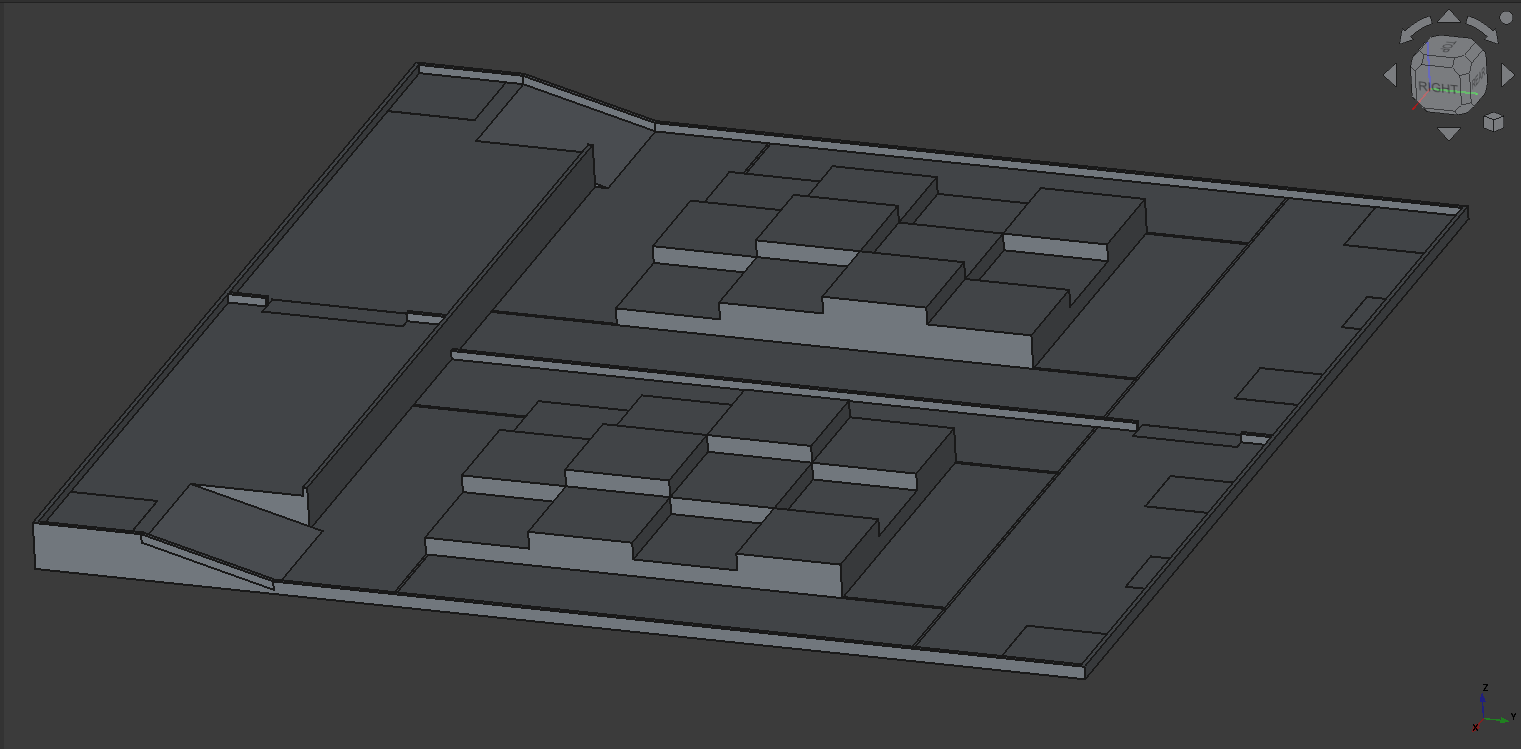
\includegraphics[width=\textwidth]{field-model-freecad.png}
    \caption{FreeCAD дээр үүсгэсэн тоглох талбайн модель}
\end{figure}
\begin{figure}[h]
    \centering
    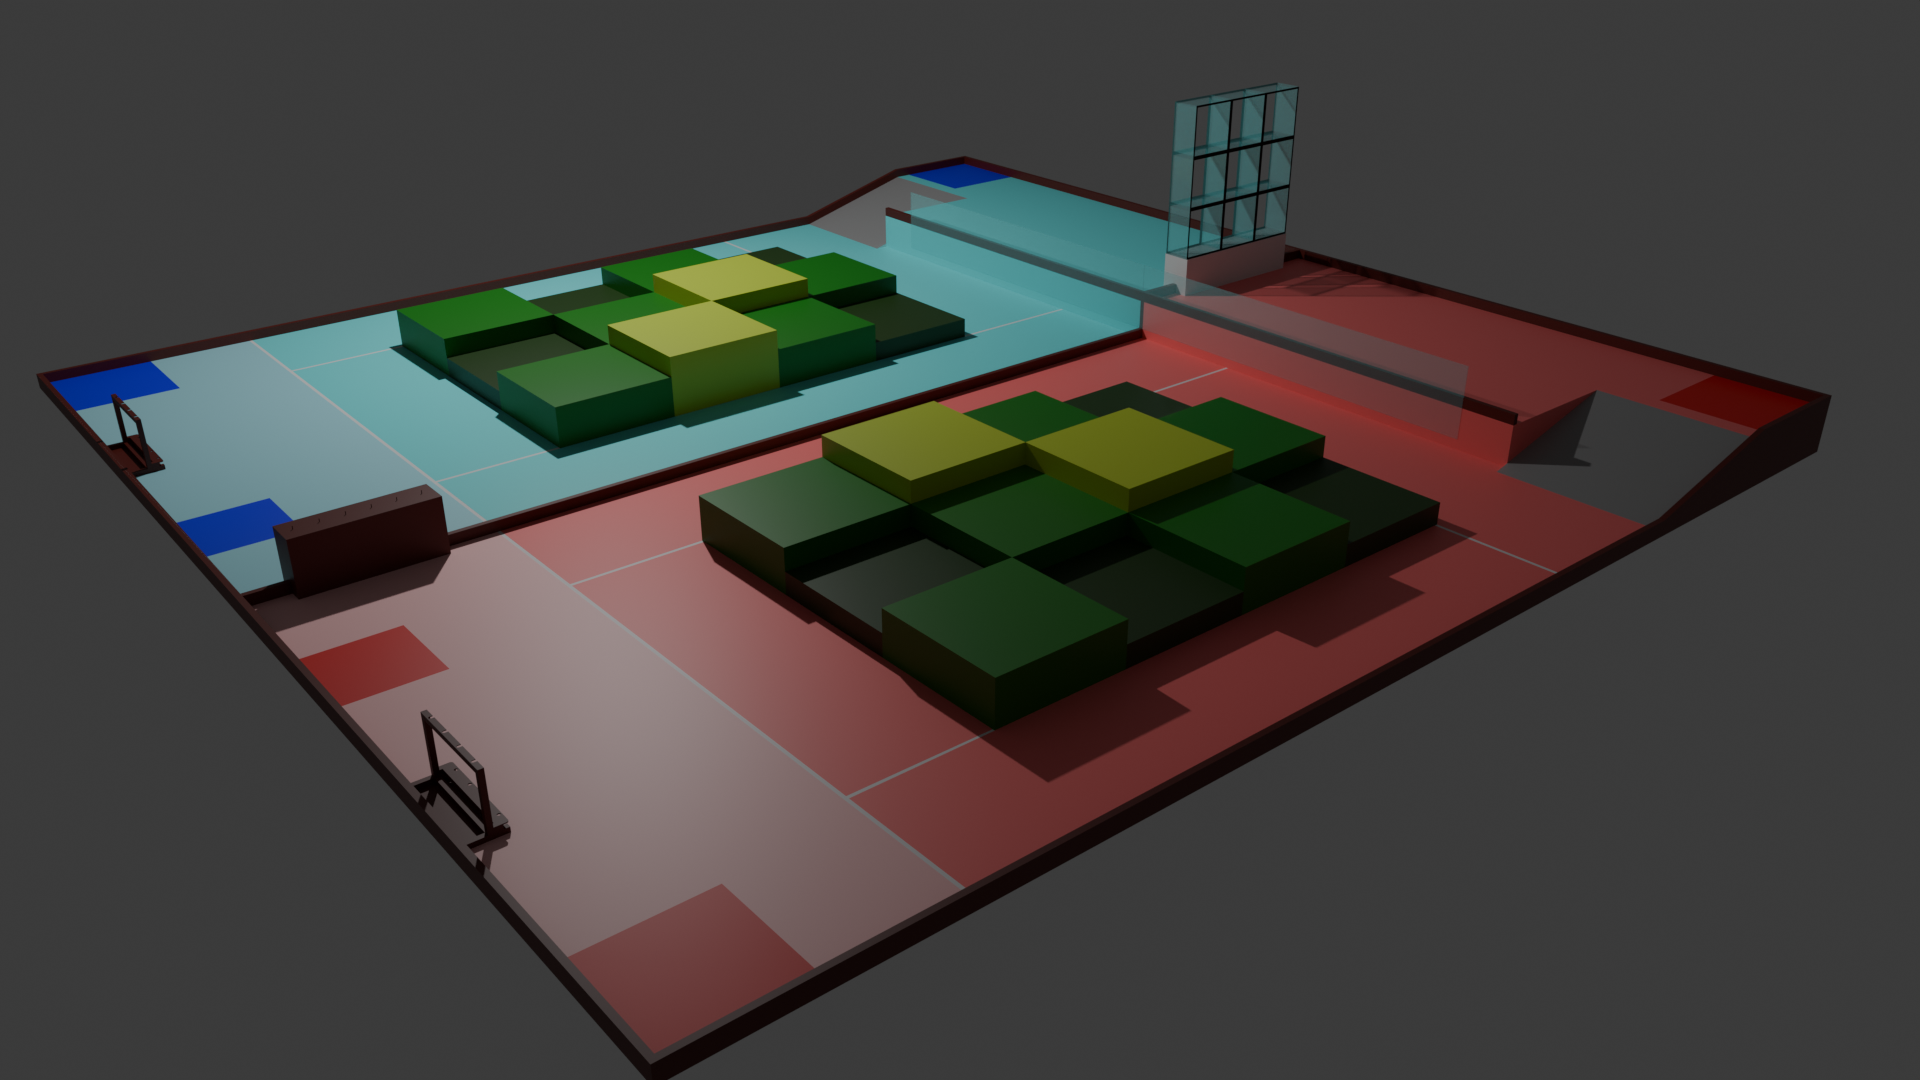
\includegraphics[width=\textwidth]{field-model-blender.png}
    \caption{Blender дээр тоглох талбайн модельд материал олгосны дараа}
    \label{fig:field-blender}
\end{figure}

\newpage

\subsection{Сургах сан}

Зураг таних машин сургалтад зориулсан Ultralytics YOLO санг ашиглан сургаж, судар таних систем боловсруулна.

Ultralytics YOLO зураг таних систем нь тухайн обьект ямар төрлийн обьект болон камерт байх байршлыг нь тогтоох боломжтой байдаг.

\begin{figure}[h]
    \centering
    
\includegraphics[width=0.5\textwidth]{ultralytics.png}
    \caption{Ultralytics YOLO лого}
    \label{fig:ultralytics}
\end{figure}

	% Argazui
	\chapter{Арга зүй}

\section{Системийн шаардлага}
Энд системийн функциональ болон функциональ бус шаардлагуудыг тодорхойлсон.

\subsection{Функциональ шаардлагууд}

\begin{itemize}
	\item ФШ-01 --- R2 робот нь жадны үзүүр авч, R1 роботтой хамт зэвсгээ угсрах шаардлагатай.
	\item ФШ-02 --- R2 робот нь мэйхуа ойг даван туулах бөгөөд, дор хаяж нэг судар авч гарах шаардлагатай.
	\item ФШ-03 --- R2 робот нь икс окс тавиурт авч ирсэн судараа байрлуулах шаардлагатай.
\end{itemize}

\subsection{Функциональ бус шаардлагууд}

\subsubsection{Программ хангамжийн шаардлагууд}
\begin{itemize}
	\item ФБШ-ПХ-01 --- R2 робот нь секундэд 10 удаа камераар авсан датаг шүүж, камерт үзэгдэх обьектуудын байршлыг тогтоох шаардлагатай.
	\item ФБШ-ПХ-02 --- R2 робот нь өөрийн байршлыг таниж, гүйцэтгэж буй явцаа ойлгосон байх шаардлагатай.
	\item ФБШ-ПХ-03 --- R2 робот нь бүрэн автоматаар ажиллах шаардлагатай.
\end{itemize}

\subsubsection{Гүйцэтгэлийн шаардлагууд}
\begin{itemize}
	\item ФБШ-Г-01 --- R2 робот нь зэвсэг угсрахдаа R1 роботтой шүргэлцэхгүй байх шаардлагатай.
	\item ФБШ-Г-02 --- R2 робот нь мэйхуа ойг давж гарах чадвартай байх шаардлагатай.
	\item ФБШ-Г-03 --- R2 робот нь судар авах, тавих болон аваад явахдаа унагахгүй байх шаардлагатай.
\end{itemize}

\newpage
\section{Системийн архитектур}

\subsection{Ерөнхий системийн архитектур}

Энэ хэсэгт ерөнхий системийн архитектур болох дүрс таних, шийдвэр гаргах гэсэн үндсэн 2 дэд систем болон тэдгээрийн R2 роботтой холбогдох схемийг илэрхийлсэн болно.

\begin{figure}[h]
    \centering
    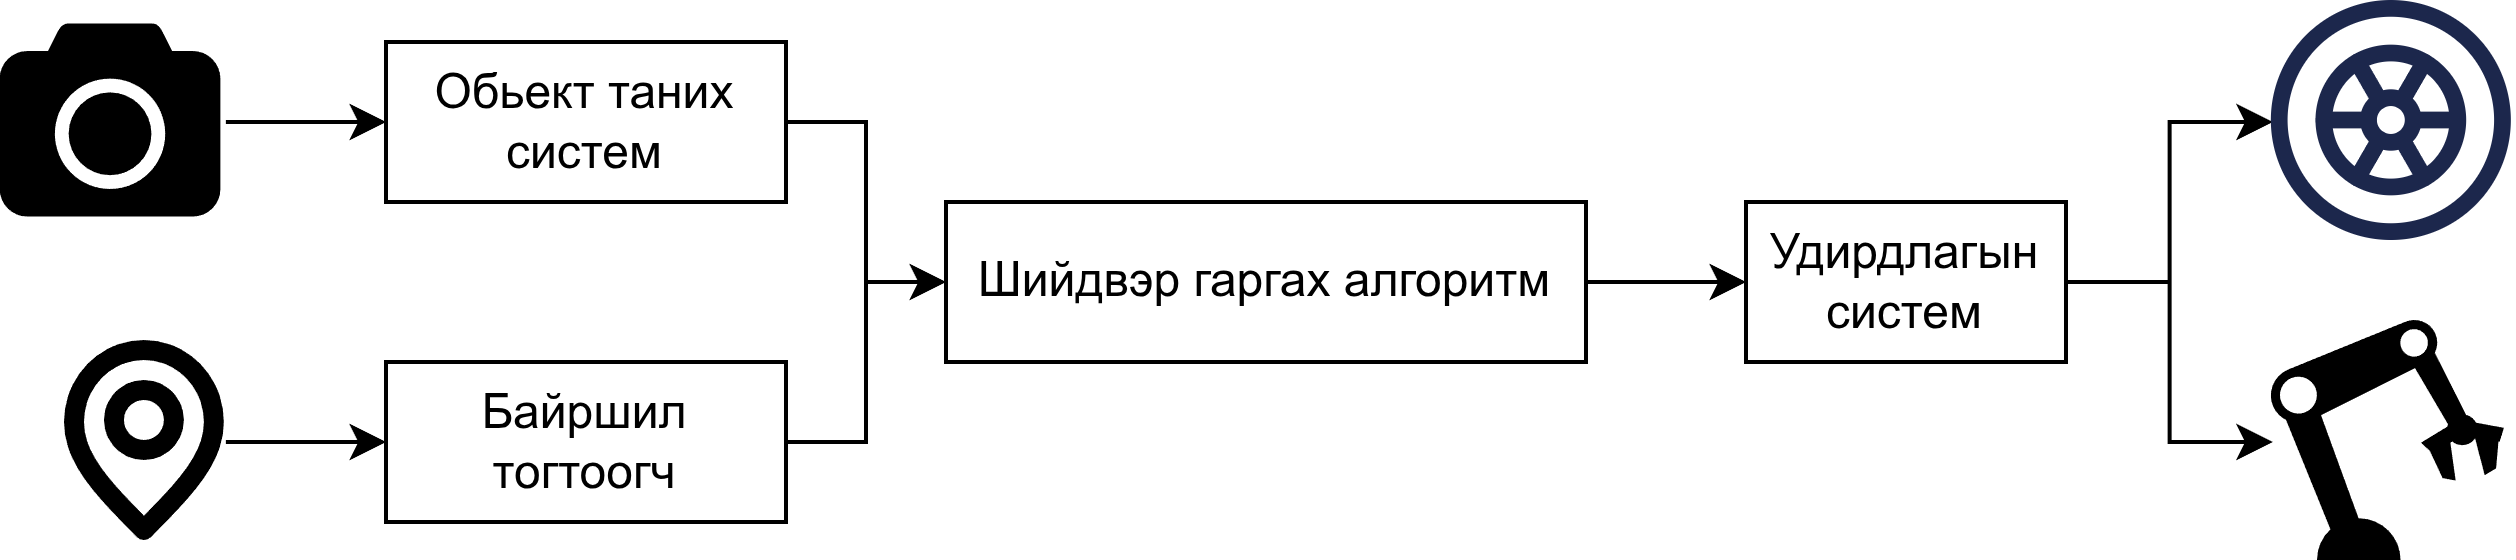
\includegraphics[width=\textwidth]{robot-structure.drawio.png}
    \caption{Ерөнхий системийн архитектур}
    \label{fig:robot-structure}
\end{figure}

\subsection{Датасет боловсруулах системийн архитектур}

Энэ хэсэгт обьект таних алгоритм сургахын тулд хэрэглэгдэх датасет боловсруулах системийн архитектурийг илэрхийлсэн болно.

\begin{figure}[h]
    \centering
    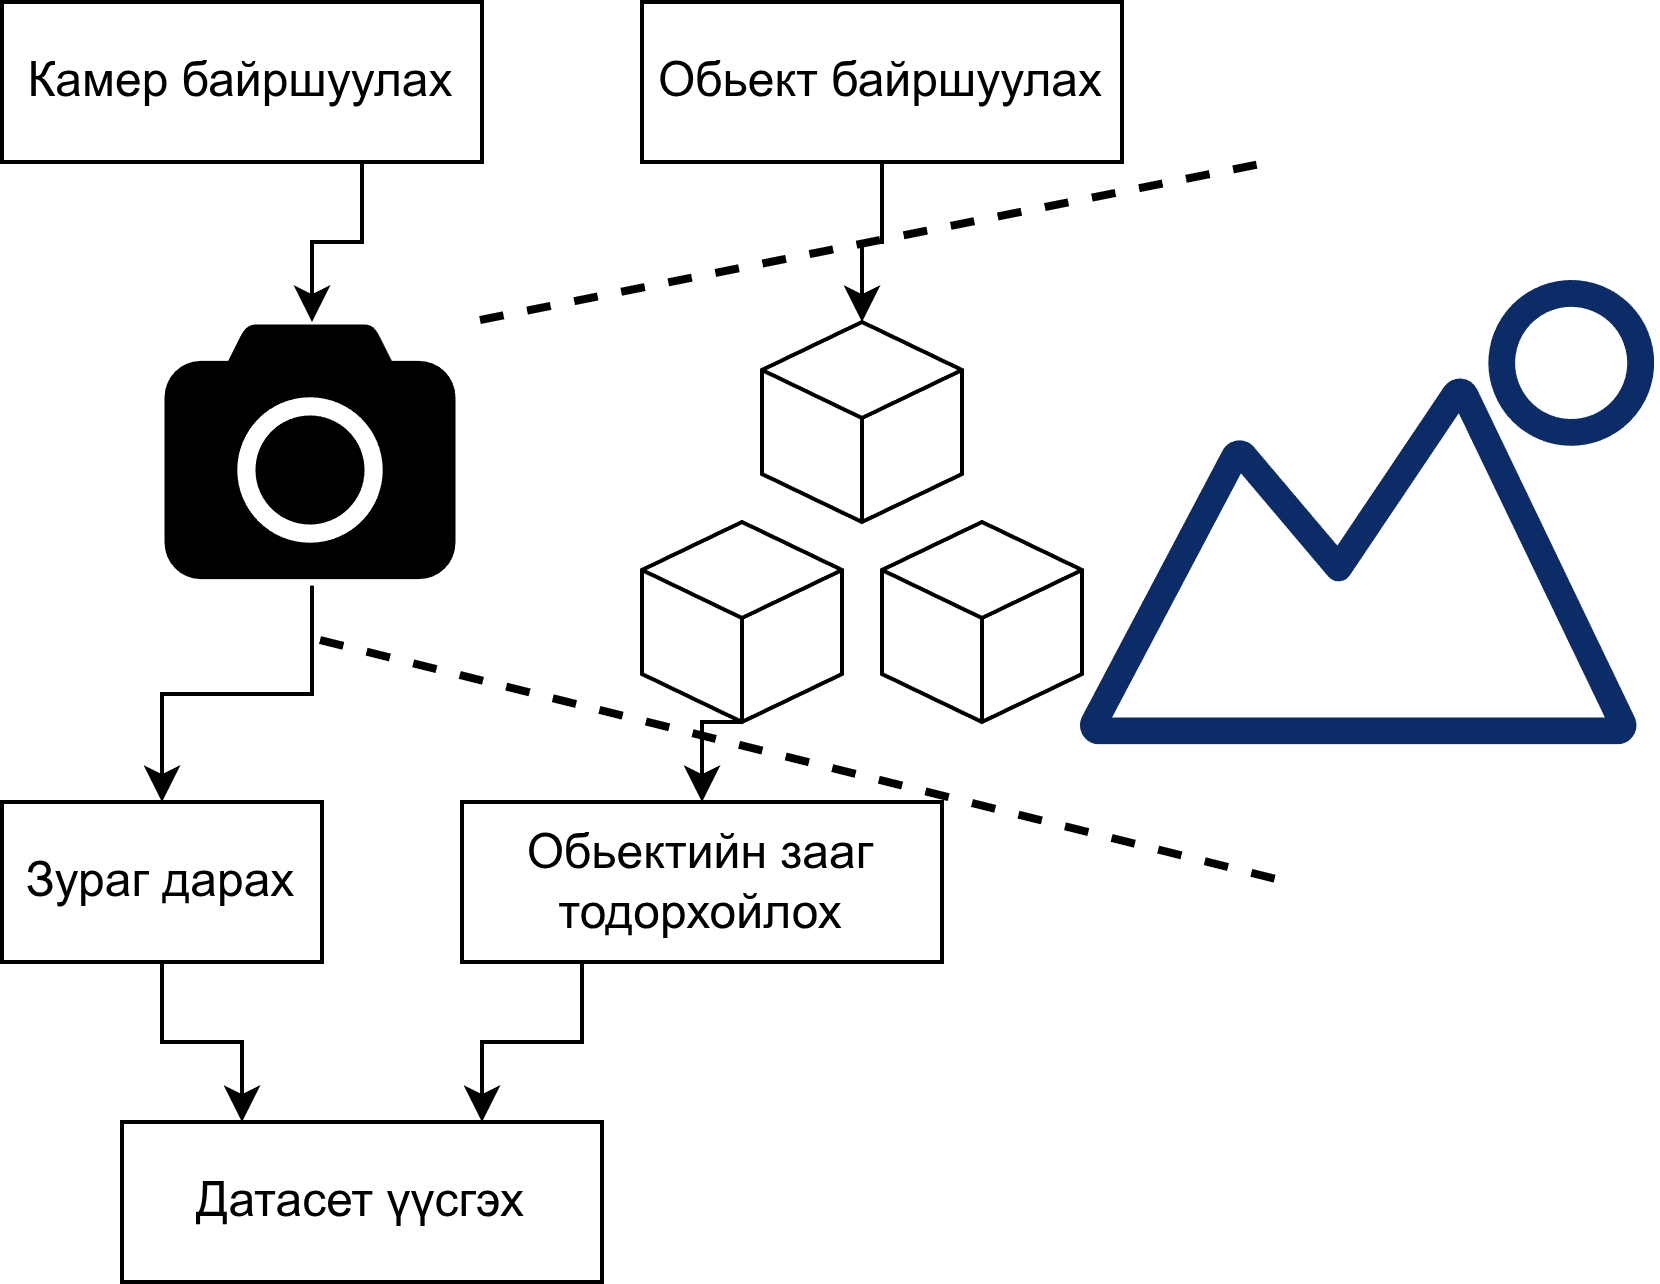
\includegraphics[width=0.7\textwidth]{dataset-generation-architecture.drawio.png}
    \caption{Датасет боловсруулах системийн архитектур}
    \label{fig:dataset-generation-architecture}
\end{figure}

\newpage
\subsection{Шийдвэр гаргах алгоритмын төлөвийн диаграм}

Шийдвэр гаргах алгоритмыг төлөвийн автоматын дагуу загварчилсан болно.
Төлөвийн диаграм нь ерөнхий 4 хэсэгт хуваагдсан болно:

\begin{enumerate}
	\item \textbf{Тохиргоо} --- Баг болон сударын байршлуудыг тохируулах хэсэг. Энд тоглогч нар гараар оролт оруулж тохируулахаар байна.
	\item \textbf{Зэвсэг угсрах} --- Жадны үзүүр олж авч, R1 робот очиж угсартал зогсож хүлээж байна. Угсарсны дараа R1 робот салгаж авах бөгөөд, үүнийг мэдрэгч ашиглан мэдэрснээр дараагийн төлөвт шилжинэ.
	\item \textbf{Судар авах} --- Мэйхуа ойруу орж, 1 ширхэг судар авч гарна. Орох болон гарахдаа R2-ийн орох болон гарах хэсгээс хэтрэхгүй байхыг анхаарах хэрэгтэй.
	\item \textbf{Судар байршуулах} --- Тулааны талбайруу орж, хоосон нүд олоод судар байршуулна. Үүний дараа дахин давтагдах бөгөөд хэрэв жадны үзүүр олсон тохиолдолд зэвсэг угсрах хэсэгт шилжих бол олдоогүй тохиолдолд судар авах хэсэгт шилжинэ.
\end{enumerate}

\begin{figure}[h]
    \centering
    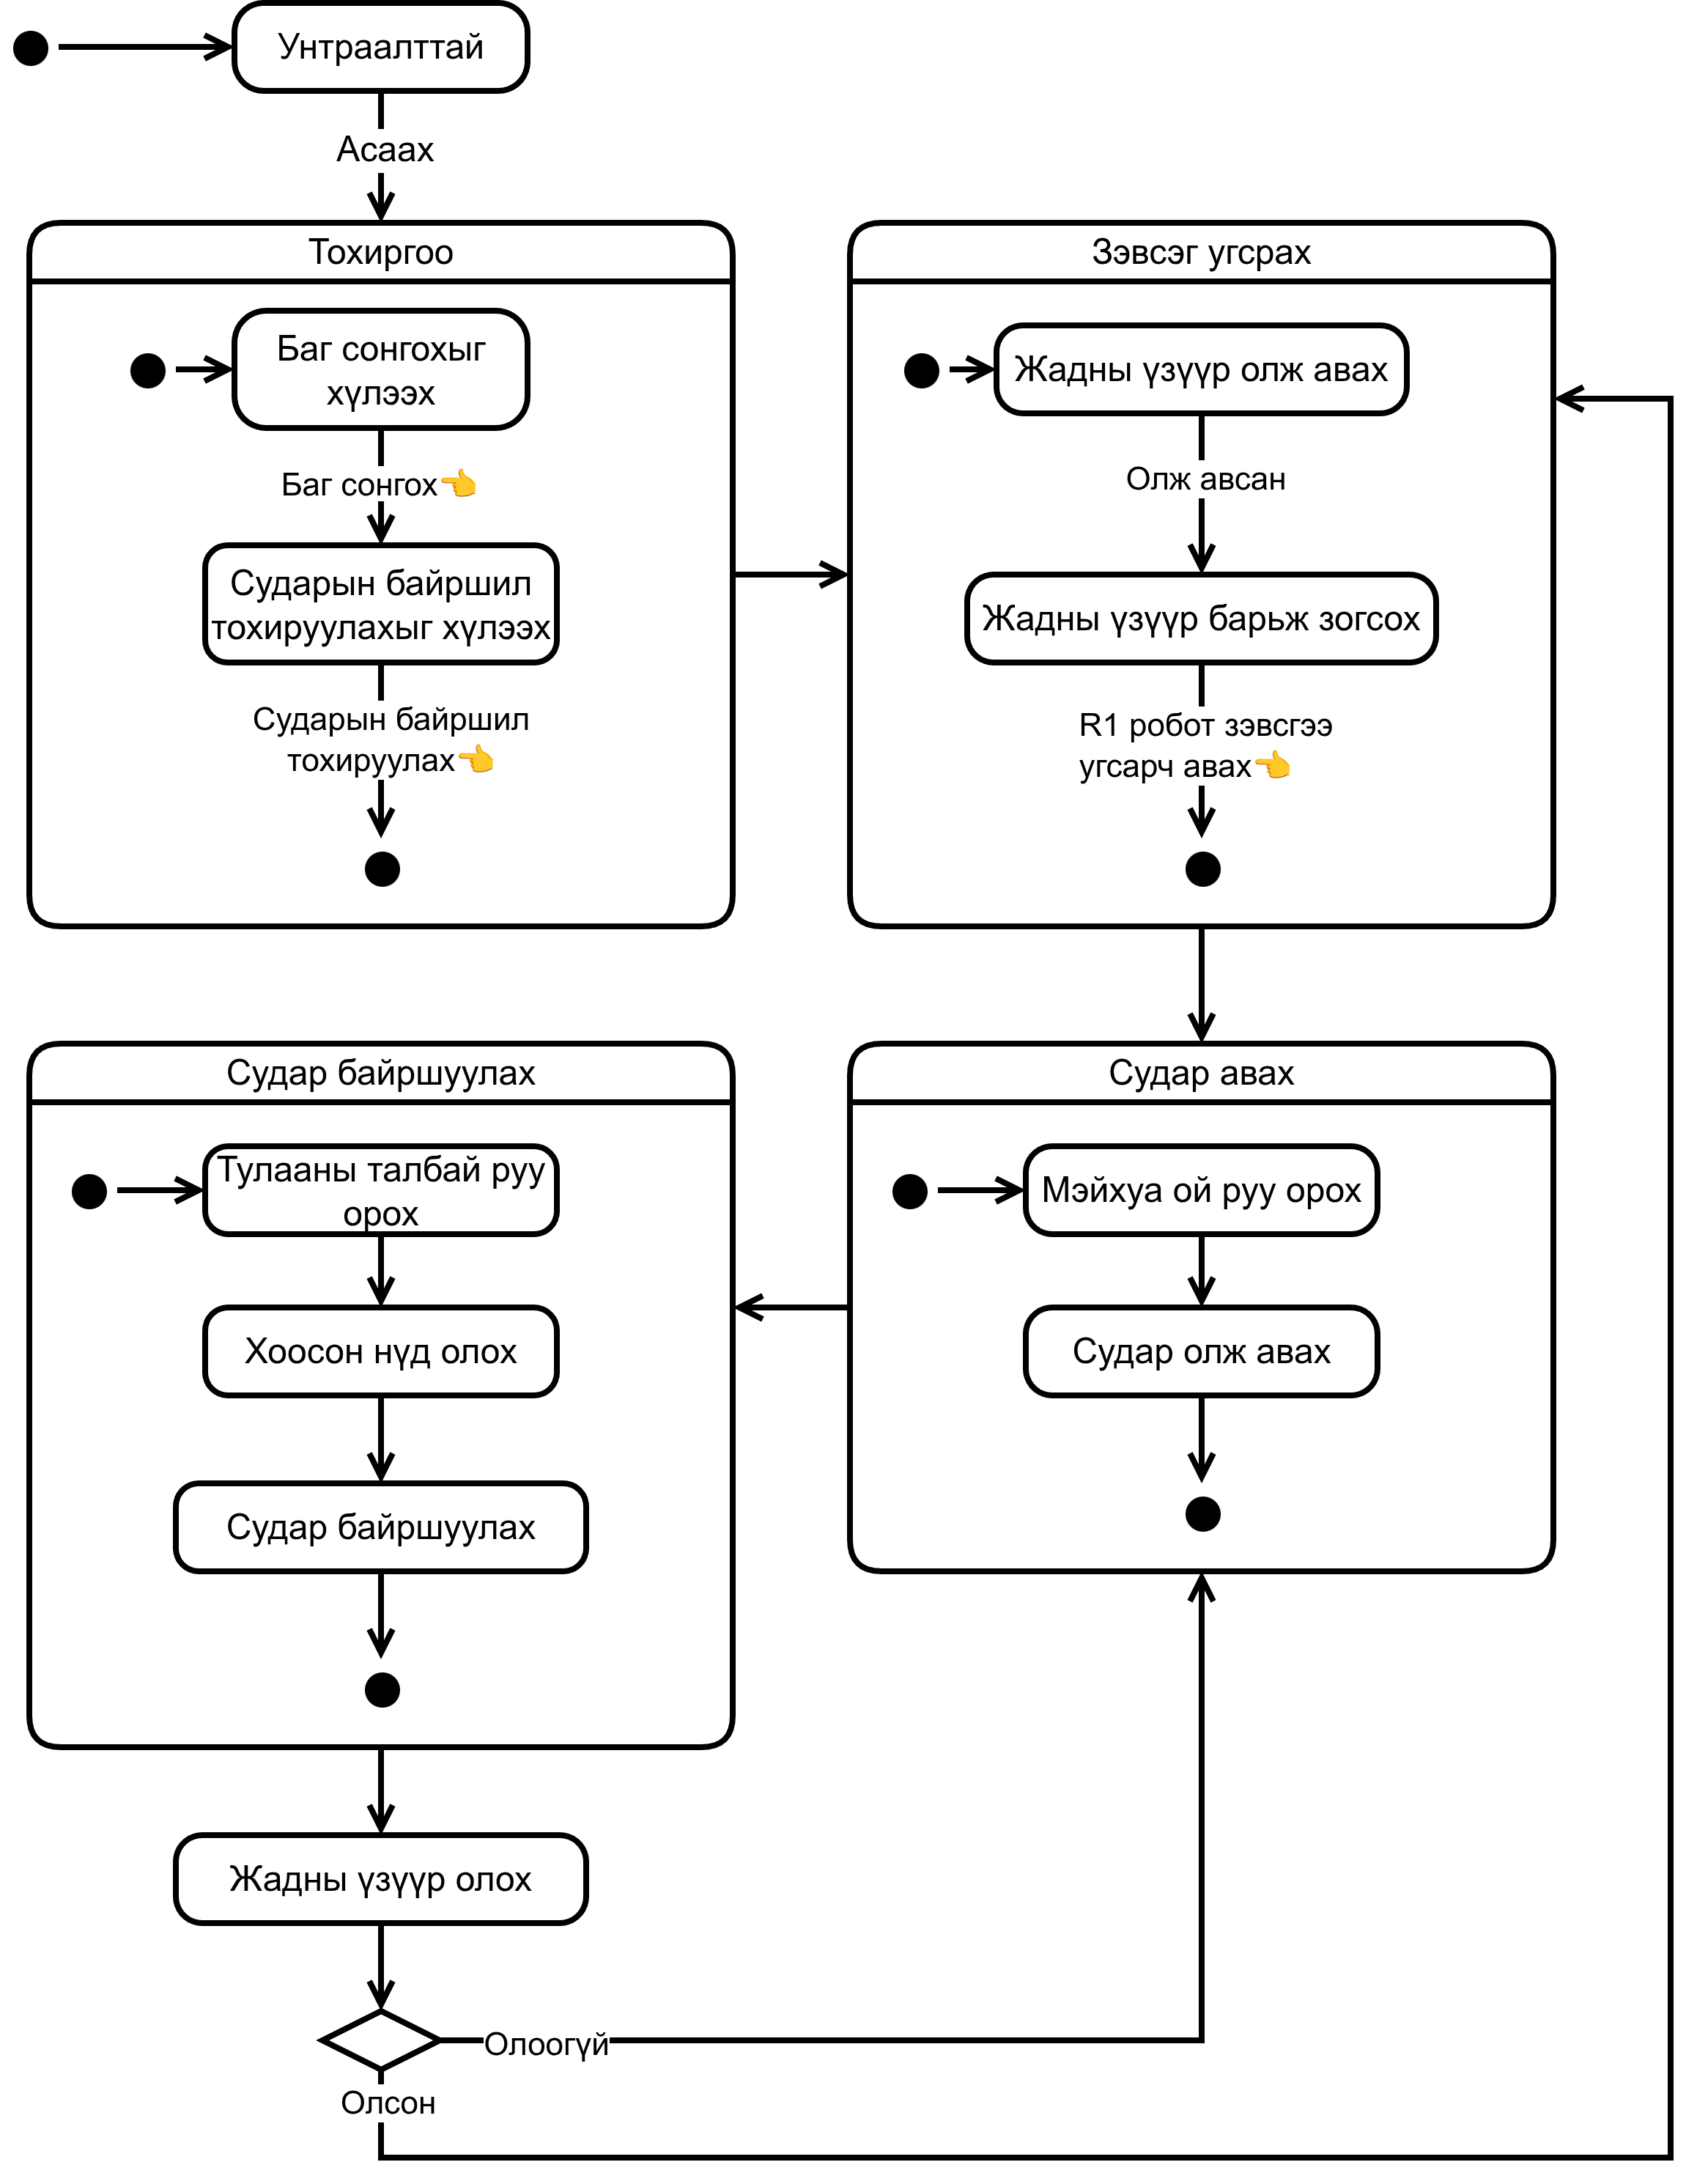
\includegraphics[width=0.7\textwidth]{state-diagram.drawio.png}
    \caption{Шийдвэр гаргах алгоритмын төлөвийн диаграм}
    \label{fig:decision-state-diagram}
\end{figure}

\newpage
\section{Обьект таних алгоритм сургалт}

R2 робот Мейхуан ойгоор явахдаа дор хаяж нэг судар авах хэрэгтэй бөгөөд, энэ судар нь икс окс тоглох гол зорилгыг биелүүлж өгдөг тул хамгийн чухал хэсэг болж өгсөн.

\subsection{Симуляцийн орчин бүрдүүлэх}

\subsubsection{Тоглох талбайн модель үүсгэх}

Датасет үүсгэхэд зориулагдсан симуляцийн орчинг бүрдүүлэх зорилготойгоор тоглох талбайн моделийг загварчилсан.
Энэхүү моделийн зураг төслийг \Robocon{} тэмцээний дүрэмд хавсаргасан зурагнаас сэдэвлэн үүсгэсэн \cite{robocon2026rulebook}.

\begin{figure}[h]
    \centering
    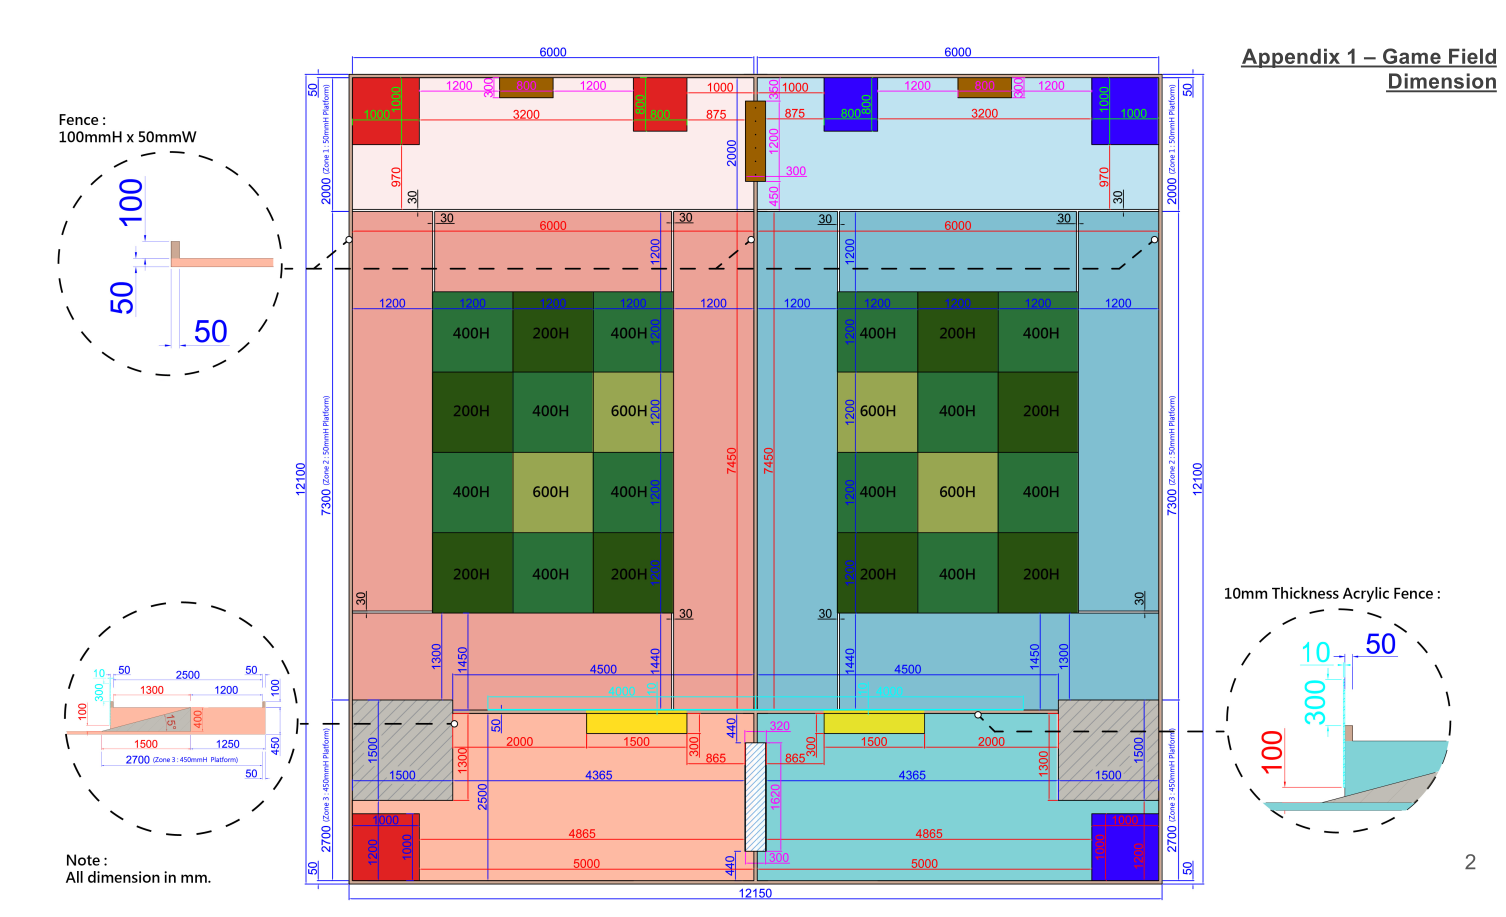
\includegraphics[width=0.7\textwidth]{robocon-field-blueprint.png}
    \caption{\Robocon{} тэмцээний дүрэмд хавсаргасан зураг төсөл \cite{robocon2026rulebook}}
    \label{fig:field-blueprint}
\end{figure}

Үүнийг загварчлахад FreeCAD болон Blender ашигласан.
FreeCAD нь геометрийн параметрууд ашиглан загварчилдаг бөгөөд, Робокон тэмцээний дүрэмд хавсаргасан тоглох талбайн зураг төслийг хавсаргасан байсан бөгөөд, үүний дагуу моделоо үүсгэсэн болно.

Моделоо үүсгэсний дараа Blender ашиглаж, өнгө болон материал өгсөн бөгөөд, энэ нь цаашлан Unity-руу моделоо оруулахад хэрэглэсэн болно.

\begin{figure}[h]
    \centering
    \begin{minipage}{0.45\textwidth}
        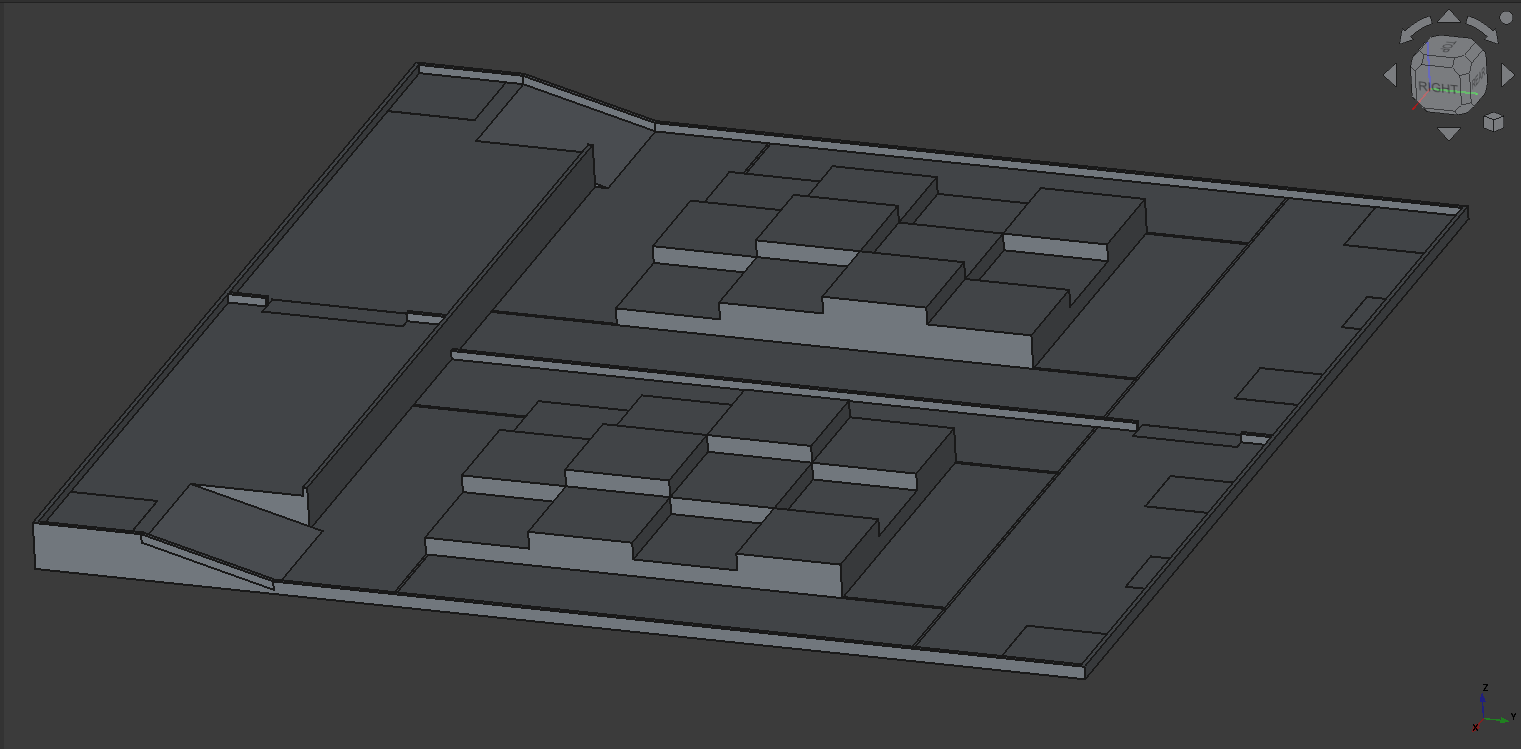
\includegraphics[width=\linewidth]{field-model-freecad.png}
        \caption{\Robocon{} тэмцээний тоглох талбайн модель}
        \label{fig:field-model-freecad}
    \end{minipage}
    \hfill
    \begin{minipage}{0.45\textwidth}
        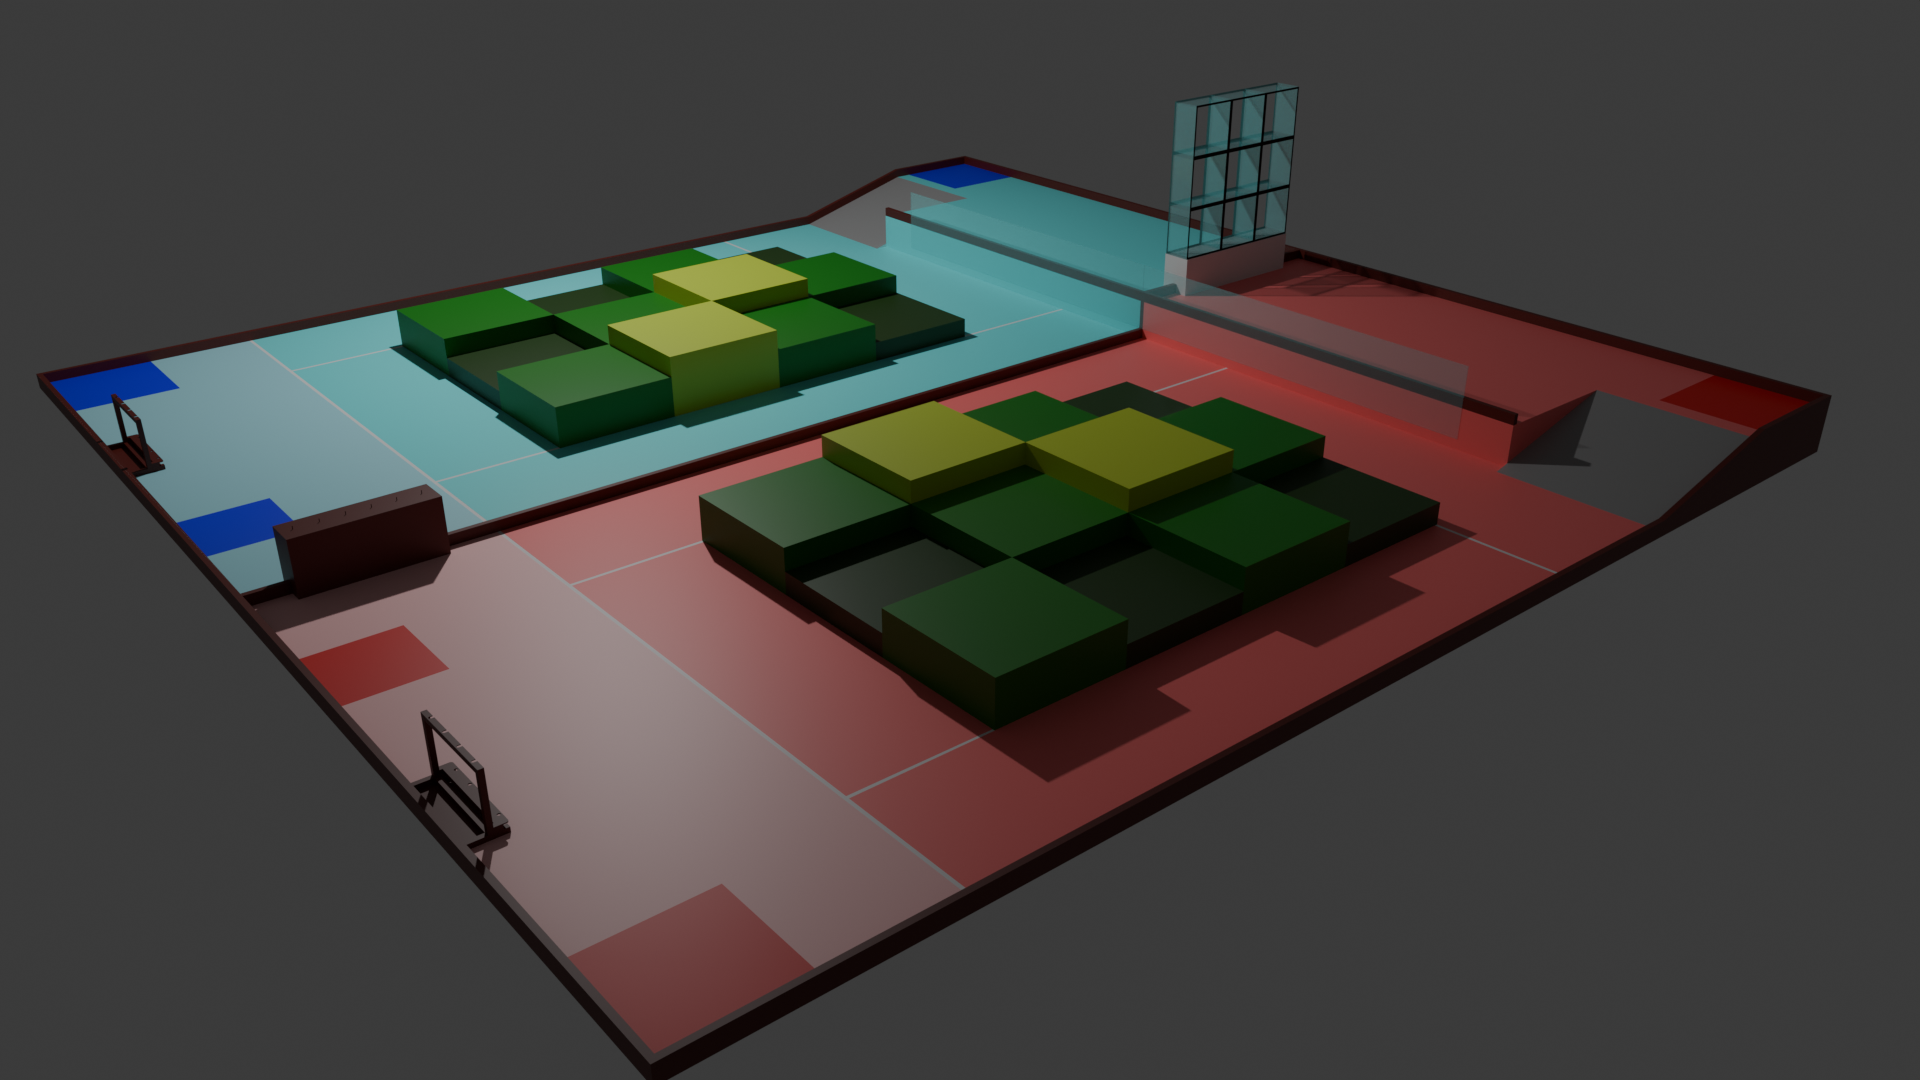
\includegraphics[width=\linewidth]{field-model-blender.png}
        \caption{Материал олгосны дараах \Robocon{} тэмцээний тоглох талбайн модель}
        \label{fig:field-model-blender}
    \end{minipage}
\end{figure}

\newpage
\subsection{Обьект таниулах датасет үүсгэх}

Датасет үүсгэхэд дор хаяж 100 зураг хэрэгтэй бөгөөд, их байх тусам үр дүнтэй байдаг тул симуляцийн орчинд үүсгэхээр Unity видео тоглоомын хөдөлгүүрийг ашигласан болно.

\subsubsection{Датасет үүсгэх код}

Датасет үүсгэхэд төрөл бүрийн өнцгөөс сударын зургуудыг авах хэрэгтэй болсон. Үүнд:
\begin{enumerate}
    \item Тоглогчийн хөдөлгөөний код
    \item Камер байршуулах код
    \item Датасет үүсгэх код
\end{enumerate}
хэмээн 3 ангилж бичсэн.

\subsubsection{Тоглогчийн хөдөлгөөний код}

Энэ нь энгийн бөгөөд тухайн тоглогч өөрийн байршлаа сольж, зураг авах тохиромжтой байрлалд очиход зориулагдсан билээ.

\subsubsection{Камер байршуулах код}

Датасет үүсгэхэд сударуудыг төрөл бүрийн өнцгөөс авсан зураг шаардлагатай бөгөөд, үүнд зориулсан камерийн дурын байршилд байрлуулах код бичсэн юм.
Энэ нь тоглогчийн байршлаас өгөгдсөн хүрээнд дурын зай, өнцөгт байрлах бөгөөд, зураг болгон дурын өнцөгт байрлуулсан байх нь үр дүнг нэмэгдүүлдэг.

\subsubsection{Датасет үүсгэх код}

Датасет үүсгэх код нь камер байршуулах код камер байршуулах бүрт ажиллах бөгөөд, энэ нь камерийн дүрсийг файлд хадгалж, мөн дүрсэд агуулагдах, сударуудын байрлалыг тооцоолж, камерт ямархуу зай эзэлж буйг тооцоолон, хариултуудыг үүсгэдэг.

Симуляцийн орчинд судар болгоны байршил нь тоглоомын ертөнцийн зүгээс өгөгдсөн байдаг тул үүнийг камерийн зүгээс харагдах байршил болгон хувиргах тооцоолол хийдэг.

	
	% Ur dun
	\chapter{Үр дүн}

\section{Обьект таних алгоритм}

	% Nomzui
	\bibliographystyle{plain}
	\bibliography{refs}

\end{document}
